\newpage
\section{Diagrammi dei packages e delle classi}

\subsection{Introduzione}
Questa sezione racchiude la descrizione dei diagrammi dei packages, progettati tramite un approccio top-down.\\ \textbf{N.B.: raggiunto il sub-package minimo, si procederà con la descrizione delle classi implementate al suo interno}.\\
Considerando l'approccio adottato e il particolare applicativo realizzato con un pattern a microservizi, il team non si discosterà dalla nomenclatura tradizionale di \textit{Classe}, intesa come una categoria di entità in grado di svolgere uno specifico compito. Nei diagrammi delle classi del back-end, è rappresentato graficamente come classe, ciò che in realtà è un microservizio. I suoi metodi mostrano l'interfaccia da esso esposta, mentre i campi dati saranno presenti solo nell'implementazione del microservizio.\\
Trattandosi di una progettazione con un livello di dettaglio intermedio, le classi non verranno definite, bensì verrà data una descrizione della loro funzionalità, lo scopo e le relazioni che intercorrono con le altre classi. Ogni componente individuato, quindi, verrà descritto adottando il seguente schema:
\begin{itemize}
	\item \textbf{Padre}: indica il package padre che contiene il componente in analisi;
	
	\item \textbf{Descrizione}: fornisce una breve descrizione riguardo funzionalità e scopo del componente;
	
	\item \textbf{Relazioni d'uso con altri componenti}: indica le eventuali varie relazioni d'uso con altri componenti, interne o esterna al package in analisi;
	
	\item \textbf{Package/classi contenuti/e}: elenco dei package e/o delle classi eventualmente contenuti dal componente in analisi.
\end{itemize}
L'applicativo \progetto\ è strutturato, come di consueto, in un lato front-end ed un lato back-end, come mostrato dal diagramma seguente:

\begin{figure}[H]
	\centering
	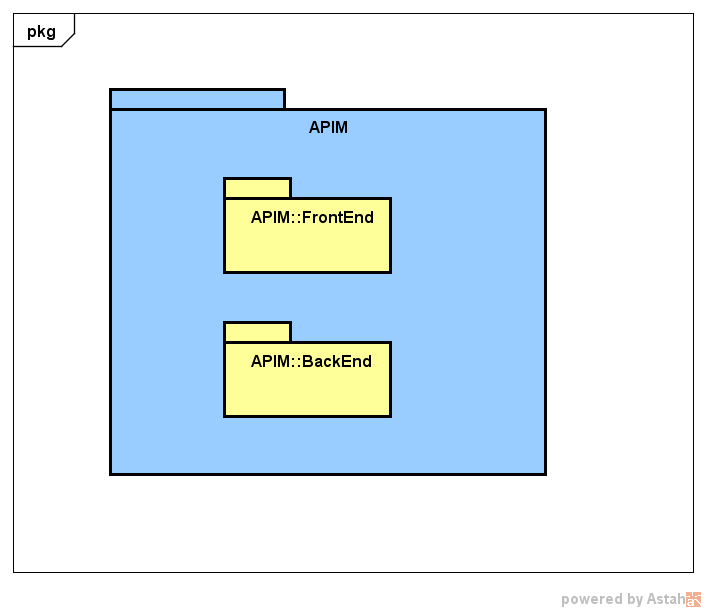
\includegraphics
	[width=0.7\linewidth]
	{UML/DiagrammiPackage/APIM.png}
	\caption{Package APIM}
\end{figure}

\newpage
\subsection{Front-end}
Nella parte front-end sono presenti i package \textit{node\_modules} e \textit{App}, che derivano dall'architettura dei componenti e framework scelti (AngularJS).

\begin{figure}[H]
	\centering
	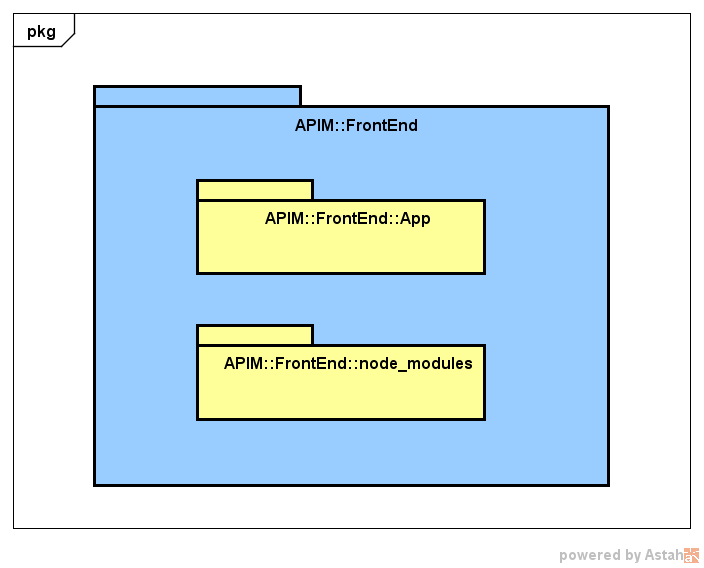
\includegraphics
	[width=0.7\linewidth]
	{UML/DiagrammiPackage/FrontEnd.png}
	\caption{Package APIM::FrontEnd}
\end{figure}

\begin{itemize}
	\item \textbf{Padre}: APIM;
	
	\item \textbf{Descrizione}: package contenente le componenti del front-end dell'applicazione;
	
	\item \textbf{Package contenuti}:
		\begin{itemize}
			\item \textbf{\textit{node\_modules}}: package contenente i riferimenti alle librerie esterne di JavaScript;
			
			\item \textbf{\textit{App}}: package contenente le componenti principali dell'applicazione.
		\end{itemize}
\end{itemize}

\subsubsection{node\_modules}
\begin{itemize}
	\item \textbf{Padre}: FrontEnd;
	
	\item \textbf{Descrizione}: package che raccoglie le librerie esterne di JavaScript, installate tramite \textit{npm} di Node.js, e fornisce le funzionalità necessarie alla parte di front-end dell'applicazione;
	
	\item \textbf{Relazioni d’uso con altri componenti}: questo package si relaziona con i \textit{controllers} presenti nel sub-package \textit{Controllers} del package \textit{App}.
\end{itemize}

\subsubsection{App}

\begin{figure}[H]
	\centering
	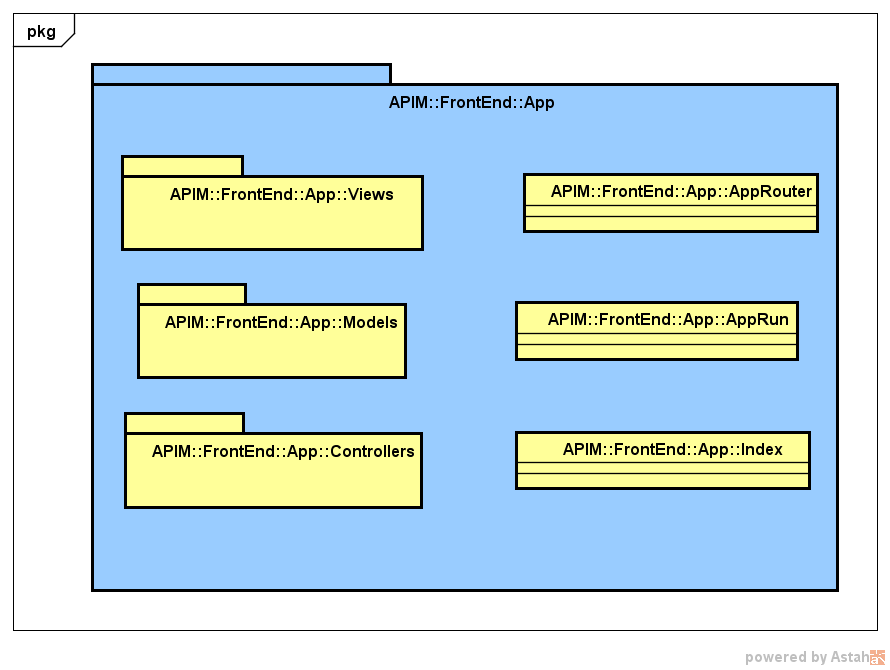
\includegraphics
	[width=0.7\linewidth]
	{UML/DiagrammiPackage/app.png}
	\caption{Package APIM::FrontEnd::App}
\end{figure}

\begin{itemize}
	\item \textbf{Padre}: FrontEnd;
	
	\item \textbf{Descrizione}: package che raccoglie le componenti principali del front-end dell'applicazione web, secondo il pattern architetturale Model-View-Controller (MVC);
	
	\item \textbf{Relazioni d’uso con altri componenti}: questo package si relaziona con le librerie presenti nel sub-package \textit{node\_modules} del package padre;
	
	\item \textbf{Package contenuti}:
		\begin{itemize}
			\item \textbf{\textit{Views}}: package contenente le \textit{views} del front-end dell'applicazione;
			
			\item \textbf{\textit{Models}}: package contenente i \textit{models} del front-end dell'applicazione;
			
			\item \textbf{\textit{Controllers}}: package contenente i \textit{controllers} del front-end dell'applicazione.
		\end{itemize}
	\item \textbf{Classi contenute}:
		\begin{itemize}
			
			\item \textbf{\textit{AppRun}}: classe che istanzia l'applicazione;
			
			\item \textbf{\textit{AppRouter}}: classe che gestisce i routes dell'applicazione;
			
			\item \textbf{\textit{Index}}: view generale dell'applicazione (single page app).
		\end{itemize}
\end{itemize}

\paragraph{AppRun}

\begin{itemize}
	\item \textbf{Padre}: App;
	
	\item \textbf{Descrizione}: classe che istanzia l'applicazione e che viene utilizzata per indicare le dipendenze tra l'applicazione e i packages esterni.
\end{itemize}

\paragraph{AppRouter}

\begin{itemize}
	\item \textbf{Padre}: App;
	
	\item \textbf{Descrizione}: classe che gestisce i routes dell'applicazione al fine di associare ad ogni route un controller e una view (associa un URL alle varie view dell'applicazione).
\end{itemize}

\paragraph{Index}

\begin{itemize}
	\item \textbf{Padre}: App;
	
	\item \textbf{Descrizione}: classe che rappresenta la view generale dell'applicazione e che contiene gli elementi che saranno presenti in ogni pagina dell'applicazione.
\end{itemize}

\paragraph{Views}

\begin{figure}[H]
	\centering
	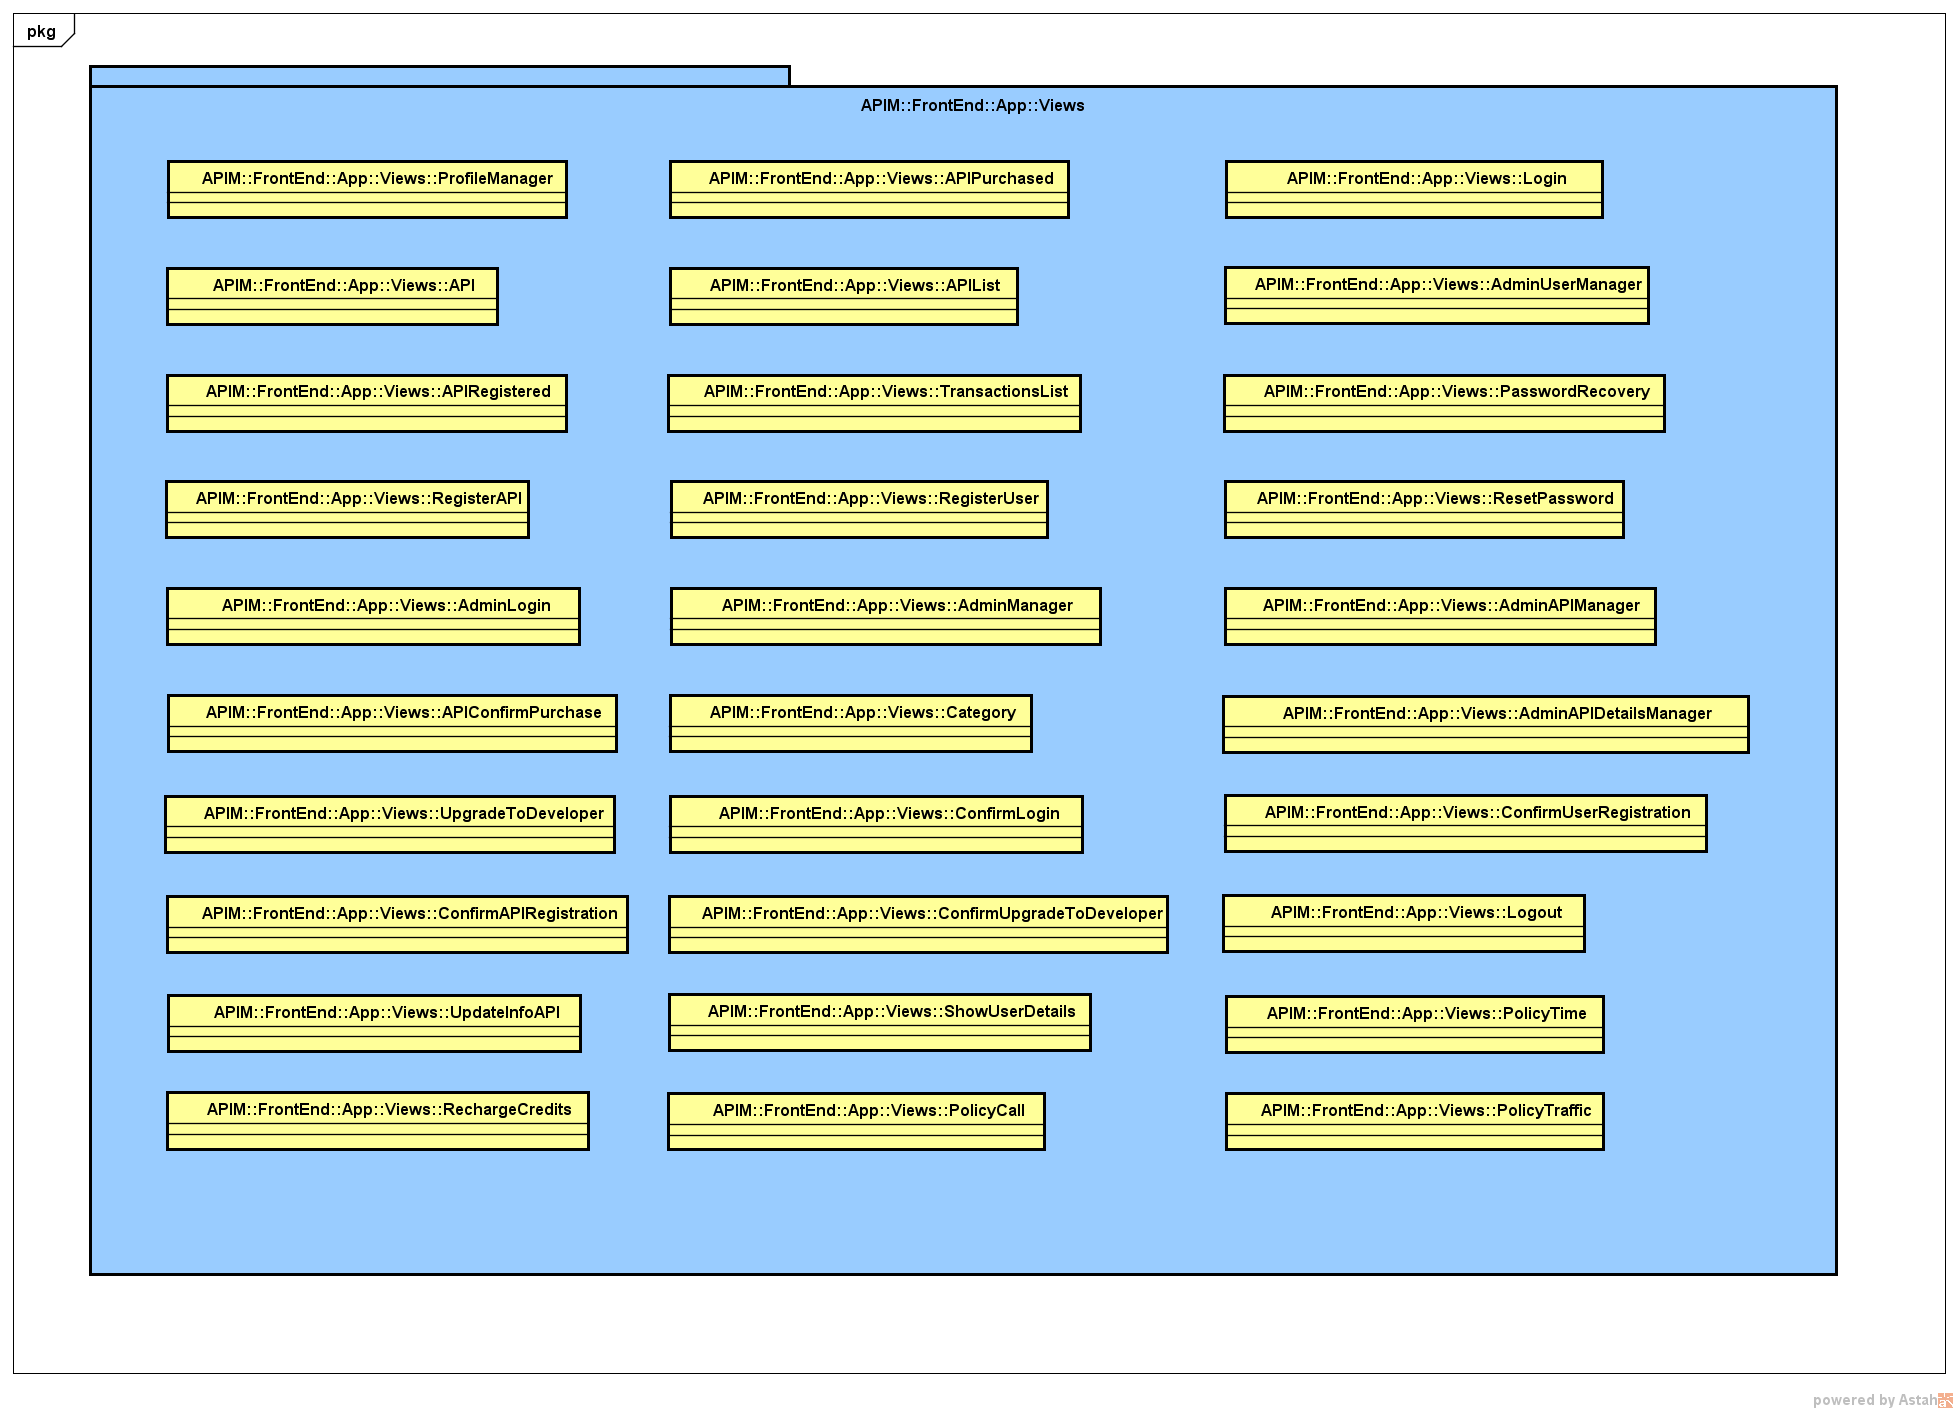
\includegraphics
	[width=0.7\linewidth]
	{UML/DiagrammiPackage/views.png}
	\caption{Package APIM::FrontEnd::App::Views}
\end{figure}

\begin{itemize}
	\item \textbf{Padre}: App;
	
	\item \textbf{Descrizione}: package contenente tutte le classi che rappresentano i vari template HTML per le pagine web dell'applicazione;
	
	\item \textbf{Relazioni d’uso con altri componenti}: questo package si relaziona con i \textit{controllers} presenti nel package \textit{Controllers};
	
	\item \textbf{Classi contenute}:
	\begin{itemize}
		\item \textbf{\textit{RegisterUser}}: view contenente il form dedicato alla registrazione di un utente, il quale può inserire i campi necessari e registrarsi così alla piattaforma. Contiene, inoltre, un link alla pagina di login.\\
		Si relaziona con le seguenti componenti: \textit{UserRegistrationController}.
		
		\item \textbf{\textit{Login}}: view contenente il form necessario affinchè l'utente possa effettuare il login ed autenticarsi al sistema. Contiene, inoltre, un link alla pagina di registrazione e uno alla pagina per il recupero della password.\\
		Si relaziona con le seguenti componenti: \textit{LoginController}.
		
		\item \textbf{\textit{PasswordRecovery}}: view contenente il form dedicato al recupero della password di un utente, il quale può inserire l'indirizzo email e ricevere una nuova password con la quale autenticarsi al sistema. Contiene, inoltre, un link alla pagina di login.\\
		Si relaziona con le seguenti componenti: \textit{PasswordRecoveryController}.
		
		\item \textbf{\textit{API}}: view contenente i risultati della ricerca effettuata, che permette di selezionare un risultato presente al suo interno.\\
		Si relaziona con le seguenti componenti: \textit{SearchController}.
		
		\item \textbf{\textit{ProfileManager}}: view contenente le informazioni del profilo personale di un utente registrato. Contiene, inoltre, l'informazione relativa al saldo del proprio conto virtuale.\\
		Si relaziona con le seguenti componenti: \textit{ProfileManagerController}.
		
		\item \textbf{\textit{ResetPassword}}: view contenente il form dedicato al cambio di password di un utente autenticato, il quale può inserire la nuova password che intende utilizzare per i futuri login al sistema.\\
		Si relaziona con le seguenti componenti: \textit{ResetPasswordController}.
		
		\item \textbf{\textit{RegisterAPI}}: view contenente il form per l'inserimento di una API da parte di un utente sviluppatore. Lo sviluppatore può inserire tutti i dati relativi al microservizio che intende esporre sul marketplace.\\
		Si relaziona con le seguenti componenti: \textit{APIRegistrationController}.
		
		\item \textbf{\textit{PolicyCall}}: view contenente le informazioni relative alla policy per chiamate.\\
		Si relaziona con le seguenti componenti: \textit{PolicyCallController}.
		
		\item \textbf{\textit{PolicyTime}}: view contenente le informazioni relative alla policy per tempo.\\
		Si relaziona con le seguenti componenti: \textit{PolicyTimeController}.
		
		\item \textbf{\textit{PolicyTraffic}}: view contenente le informazioni relative alla policy per traffico dati.\\
		Si relaziona con le seguenti componenti: \textit{PolicyTrafficController}.
		
		\item \textbf{\textit{APIRegistered}}: view contenente le informazioni di una API registrata sulla piattaforma.\\
		Si relaziona con le seguenti componenti: \textit{APIRegisteredController}.
		
		\item \textbf{\textit{APIPurchased}}: view contenente le informazioni delle API acquistate da un cliente della piattaforma \progetto.\\
		Si relaziona con le seguenti componenti: \textit{APIPurchasedController}.
		
		\item \textbf{\textit{APIList}}: view contenente l'elenco delle API disponibili sul marketplace \progetto.\\
		Si relaziona con le seguenti componenti: \textit{APIListController}.
		
		\item \textbf{\textit{TransactionsList}}: view contenente l'elenco delle transazioni effettuate da un utente sul marketplace \progetto.\\
		Si relaziona con le seguenti componenti: \textit{TransactionsListController}.
				
		\item \textbf{\textit{APIConfirmPurchase}}: view contenente la conferma di un acquisto di una API.\\
		Si relaziona con le seguenti componenti: \textit{APIConfirmPurchaseController}.
				
		\item \textbf{\textit{AdminManager}}: view contenente le operazioni per la gestione del profilo amministratore \progetto.\\
		Si relaziona con le seguenti componenti: \textit{AdminManagerController}.
		
		\item \textbf{\textit{Category}}: view contenente l'elenco delle categoria nell'\progetto.\\
		Si relaziona con le seguenti componenti: \textit{CategoryController}.
		
		\item \textbf{\textit{ConfirmUpgradeToDeveloper}}: view contenente la conferma dell'upgrade di un utente a sviluppatore nell'\progetto.\\
		Si relaziona con le seguenti componenti: \textit{ConfirmUpgradeToDeveloperController}.
		
		\item \textbf{\textit{ConfirmLogin}}: view contenente la conferma di login all'\progetto.\\
		Si relaziona con le seguenti componenti: \textit{ConfirmLoginController}.
		
		\item \textbf{\textit{ConfirmUserRegistration}}: view contenente la conferma di registrazione all'\progetto.\\
		Si relaziona con le seguenti componenti: \textit{ConfirmUserRegistrationController}.
		
		\item \textbf{\textit{ConfirmAPIRegistration}}: view contenente la conferma di registrazione di una API all'\progetto.\\
		Si relaziona con le seguenti componenti: \textit{ConfirmAPIRegistrationController}.
		
		\item \textbf{\textit{UpgradeToDeveloper}}: view contenente il modulo per diventare sviluppatore all'interno dell'\progetto.\\
		Si relaziona con le seguenti componenti: \textit{UpgradeToDeveloperController}.
		
		\item \textbf{\textit{AdminAPIManager}}: view contenente le operazioni dell'amministratore sulle API dell'\progetto.\\
		Si relaziona con le seguenti componenti: \textit{AdminAPIManagerController}.
		
		\item \textbf{\textit{AdminAPIDetailsManager}}: view contenente le statistiche di una API dell'\progetto.\\
		Si relaziona con le seguenti componenti: \textit{AdminAPIDetailsManagerController}.
		
		\item \textbf{\textit{AdminUserManager}}: view contenente le operazioni di un ammistratore sugli utenti dell'\progetto.\\
		Si relaziona con le seguenti componenti: \textit{AdminUserManagerController}.
		
		\item \textbf{\textit{AdminLogin}}: view contenente il form necessario affinchè l'amministratore possa effettuare il login ed autenticarsi al sistema.\\
		Si relaziona con le seguenti componenti: \textit{AdminLoginController}.
		
		\item \textbf{\textit{Logout}}: view contenente la conferma di logout dall'\progetto.\\
		Si relaziona con le seguenti componenti: \textit{LogoutController}.
		
		\item \textbf{\textit{UpdateInfoAPI}}: view contenente il form dedicato modifica delle informazioni di una API presente nel marketplace \progetto.\\
		Si relaziona con le seguenti componenti: \textit{UpdateInfoAPIController}.
		
		\item \textbf{\textit{RechargeCredits}}: view contenente la possibilità di scegliere quanti crediti ricaricare sul conto personale tra i tagli disponibili.\\
		Si relaziona con le seguenti componenti: \textit{RechargeCreditsController}.
		
		item \textbf{\textit{ShowUserDetalis}}: view contenente le informazioni personali di un utente visualizzabili da altri fruitori del marketplace \progetto.\\
		Si relaziona con le seguenti componenti: \textit{ShowUserDetalisController}.
		
		\item \textbf{\textit{AdminModeration}}: view contenente il form dedicato alla moderazione di un utente o di una API/microservizio da parte di un amministratore della piattaforma \progetto.\\
		Si relaziona con le seguenti componenti: \textit{AdminModerationController}.
	\end{itemize}
\end{itemize}

\paragraph{Models}

\begin{figure}[H]
	\centering
	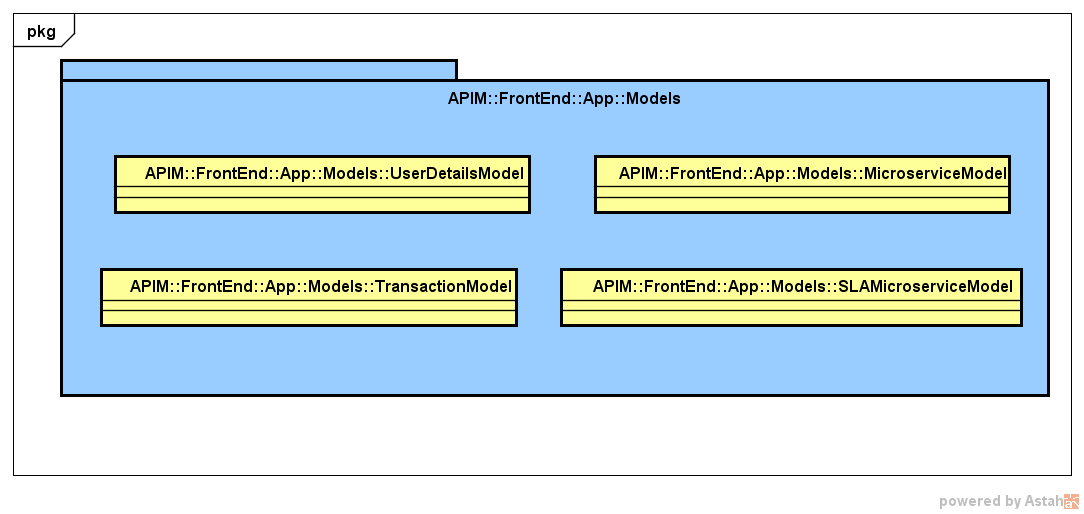
\includegraphics
	[width=0.7\linewidth]
	{UML/DiagrammiPackage/Models.png}
	\caption{Package APIM::FrontEnd::App::Models}
\end{figure}

\begin{itemize}
	\item \textbf{Padre}: App;
	
	\item \textbf{Descrizione}: package che contiene le classi che definiscono la business logic dell'applicazione;
	
	\item \textbf{Relazioni d’uso con altri componenti}: questo package si relaziona con il package \textit{Controllers};
	
	\item \textbf{Classi contenute}:
	\begin{itemize}
		\item \textbf{\textit{UserDetailsModel}}: classe che rappresenta un utente e che contiene tutte le informazioni necessarie alla presentazione del contenuto di un utente, sia nella visualizzazione che nella gestione di un profilo.\\
		Si relaziona con le seguenti componenti: \textit{LoginController}, \textit{SearchController}, \textit{ProfileManagerController}, \textit{ResetPasswordController}, \textit{PasswordRecoveryController}.
		
		\item \textbf{\textit{MicroserviceModel}}: classe che rappresenta un microservizio e che contiene tutte le informazioni necessarie alla presentazione del contenuto di un microservizio, sia nella visualizzazione che nella gestione.\\
		Si relaziona con le seguenti componenti: \textit{APIRegiteredController}, \textit{APIRegistrationController}, \textit{PolicyCall}, \textit{PolicyTime}, \textit{PolicyTraffic}, \textit{APIPurchasedController}, \textit{APIListController}.
		
		\item \textbf{\textit{TransactionModel}}:  classe che rappresenta una transazione avvenuta e che contiene tutte le informazioni necessarie alla presentazione del contenuto di una transazione, sia nella visualizzazione che nella gestione.\\
		Si relaziona con le seguenti componenti: \textit{TransactionsListController}, \textit{APIPurchasedController}.
		
		\item \textbf{\textit{SLAMicroserviceModel}}:  classe che rappresenta la SLA di un microservizio e che contiene tutte le informazioni necessarie alla presentazione del contenuto di SLA di un microservizio, sia nella visualizzazione che nella gestione.\\
		Si relaziona con le seguenti componenti: \textit{PolicyCall}, \textit{PolicyTime}, \textit{PolicyTraffic}, \textit{APIRegistrationController}.
	\end{itemize}
\end{itemize}
	
\paragraph{Controllers}

\begin{figure}[H]
	\centering
	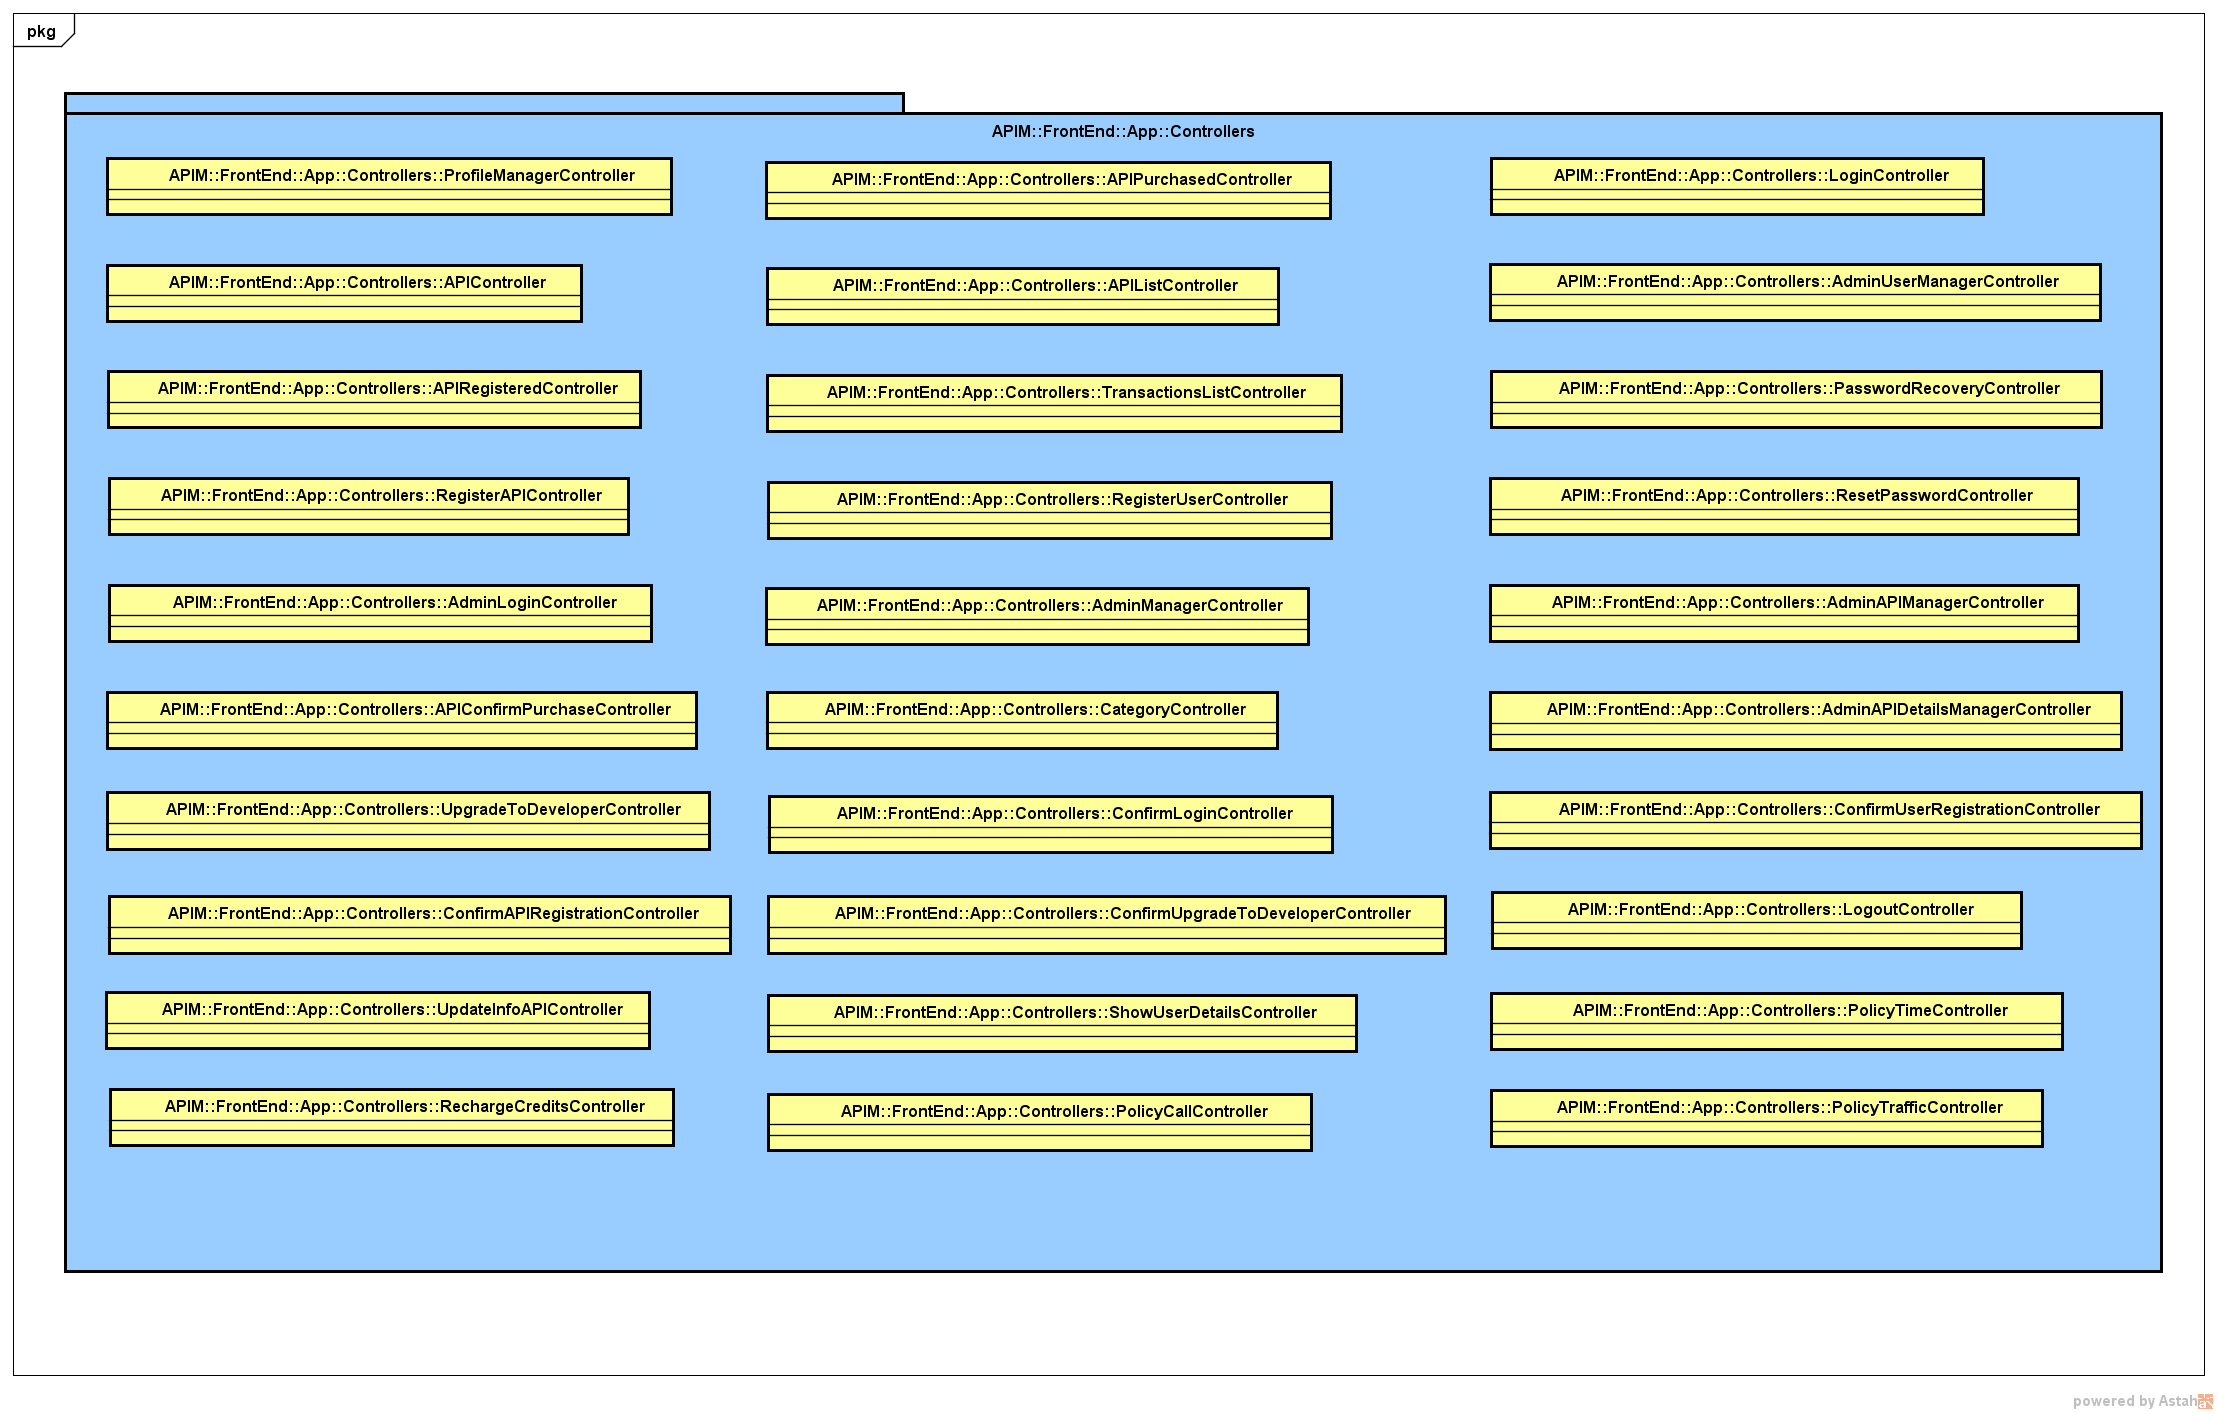
\includegraphics
	[width=0.7\linewidth]
	{UML/DiagrammiPackage/Controllers.png}
	\caption{Package APIM::FrontEnd::App::Controllers}
\end{figure}

\begin{itemize}
	\item \textbf{Padre}: App;
	
	\item \textbf{Descrizione}: package che contiene i \textit{controllers} individuati per la parte front-end
	dell'applicazione, i quali consentono la gestione delle azioni utente dell'applicazione web;
	
	\item \textbf{Relazioni d’uso con altri componenti}: questo package si relaziona con i package \textit{Views} e \textit{Models}.
	
	\item \textbf{Classi contenute}:
	\begin{itemize}
		
		\item \textbf{\textit{UserRegistrationController}}: classe che permette di gestire la registrazione di un utente al sistema, fornendone le funzionalità preposte.\\
		Si relaziona con le seguenti componenti: \textit{RegisterUser}.
		
		\item \textbf{\textit{LoginController}}: classe che permette di gestire il login di un utente alla piattaforma \progetto, fornendo le funzionalità di autenticazione al sistema, compresa la gestione di	situazioni di errore di autenticazione.\\
		Si relaziona con le seguenti componenti: \textit{UserDetailsModel}, \textit{Login}.
		
		\item \textbf{\textit{PasswordRecoveryController}}: classe che permette di gestire il ripristino della password dimenticata da un utente, fornendo tutte le funzionalità per il recupero della password dopo aver verificato l'identità dell'utente.\\
		Si relaziona con le seguenti componenti: \textit{UserDetailsModel}, \textit{PasswordRecovery}.
		
		\item \textbf{\textit{SearchController}}: classe che permette di gestire la ricerca di microservizi all'interno del marketplace \progetto, fornendo all'utente le funzionalità di ricerca tramite categorie e keywords per sviluppatori e microservizi.\\
		Si relaziona con le seguenti componenti: \textit{API}.
		
		\item \textbf{\textit{ProfileManagerController}}: classe che permette di gestire il profilo personale di un utente, fornendo le funzionalità all'utente per poter modificare i propri dati.\\
		Si relaziona con le seguenti componenti: \textit{UserDetailsModel}, \textit{ProfileManager}.
		
		\item \textbf{\textit{ResetPasswordController}}: classe che permette di gestire il cambio password di un utente autenticato al sistema, fornendo le funzionalità per il salvataggio di una nuova password.\\
		Si relaziona con le seguenti componenti: \textit{UserDetailsModel}, \textit{ResetPassword}.
		
		\item \textbf{\textit{APIRegistrationController}}: classe che permette di gestire l'inserimento di una API, fornendo tutte le funzionalità atte alla corretta esposizione di un microservizio di uno sviluppatore, utente della piattaforma \progetto.\\
		Si relaziona con le seguenti componenti: \textit{MicroserviceModel}, \textit{RegisterAPI}.
				
		\item \textbf{\textit{PolicyCallController}}: classe che permette di gestire le policy di vendita dei microservizi per chiamate.\\
		Si relaziona con le seguenti componenti: \textit{PolicyCall}, \textit{SLAMicroserviceModel}.
		
		\item \textbf{\textit{PolicyTimeController}}: classe che permette di gestire le policy di vendita dei microservizi per tempo.\\
		Si relaziona con le seguenti componenti: \textit{PolicyTime}, \textit{SLAMicroserviceModel}.
		
		\item \textbf{\textit{PolicyTrafficController}}: classe che permette di gestire le policy di vendita dei microservizi per traffico dati.\\
		Si relaziona con le seguenti componenti: \textit{PolicyTraffic}, \textit{SLAMicroserviceModel}.
		
		\item \textbf{\textit{APIRegisteredController}}: classe che permette di gestire le informazioni di una API precedentemente inserita.\\
		Si relaziona con le seguenti componenti: \textit{MicroserviceModel}, \textit{APIRegistered}.
		
		\item \textbf{\textit{APIPurchasedController}}: classe che permette di gestire l'acquisto e le relative informazioni di una API, fornendo l'API Key per l'utilizzo del cliente.\\
		Si relaziona con le seguenti componenti: \textit{APIPurchased}, \textit{MicroserviceModel}, \textit{TransactionModel}.
		
		\item \textbf{\textit{APIListController}}: classe che permette di gestire l'elenco dei microservizi presenti sul marketplace \progetto.\\
		Si relaziona con le seguenti componenti: \textit{APIList}, \textit{MicroserviceModel}.
		
		\item \textbf{\textit{TransactionsListController}}: classe che permette di gestire lo storico delle transazioni di un utente del marketplace \progetto.\\
		Si relaziona con le seguenti componenti: \textit{TransactionsList}, \textit{TransactionsModel}.
			
		\item \textbf{\textit{AdminManagerController}}: classe che permette di gestire il profilo di un amministratore della piattaforma \progetto, fornendo le funzionalità per poter modificare i propri dati e moderare utenti ed API.\\
		Si relaziona con le seguenti componenti: \textit{AdminManager}.
		%----------------------
		
		\item \textbf{\textit{CategoryController}}: classe che permette di gestire l'elenco delle categoria nell'\progetto.\\
		Si relaziona con le seguenti componenti: \textit{Category}.
		
		\item \textbf{\textit{ConfirmUpgradeToDeveloperController}}: classe che permette di gestire la conferma dell'upgrade di un utente a sviluppatore nell'\progetto.\\
		Si relaziona con le seguenti componenti: \textit{ConfirmUpgradeToDeveloper}.
		
		\item \textbf{\textit{ConfirmLoginController}}: classe che permette di gestire la conferma di login all'\progetto.\\
		Si relaziona con le seguenti componenti: \textit{ConfirmLogin}.
		
		\item \textbf{\textit{ConfirmUserRegistrationController}}: classe che permette di gestire la conferma di registrazione all'\progetto.\\
		Si relaziona con le seguenti componenti: \textit{ConfirmUserRegistration}.
		
		\item \textbf{\textit{ConfirmAPIRegistrationController}}: classe che permette di gestire la conferma di registrazione di una API all'\progetto.\\
		Si relaziona con le seguenti componenti: \textit{ConfirmAPIRegistration}.
		
		\item \textbf{\textit{UpgradeToDeveloperController}}: classe che permette di gestire il modulo per diventare sviluppatore all'interno dell'\progetto.\\
		Si relaziona con le seguenti componenti: \textit{UpgradeToDeveloper}.
		
		\item \textbf{\textit{AdminAPIManagerController}}: classe che permette di gestire le operazioni dell'amministratore sulle API dell'\progetto.\\
		Si relaziona con le seguenti componenti: \textit{AdminAPIManager}.
		
		\item \textbf{\textit{AdminAPIDetailsManagerController}}: classe che permette di gestire le statistiche di una API dell'\progetto.\\
		Si relaziona con le seguenti componenti: \textit{AdminAPIDetailsManager}.
		
		\item \textbf{\textit{AdminUserManagerController}}: classe che permette di gestire le operazioni di un ammistratore sugli utenti dell'\progetto.\\
		Si relaziona con le seguenti componenti: \textit{AdminUserManager}.
		
		\item \textbf{\textit{AdminLoginController}}: classe che permette di gestire il form necessario affinchè l'amministratore possa effettuare il login ed autenticarsi al sistema.\\
		Si relaziona con le seguenti componenti: \textit{AdminLogin}.
		
		\item \textbf{\textit{Logout}}: classe che permette di gestire la conferma di logout dall'\progetto.\\
		Si relaziona con le seguenti componenti: \textit{LogoutController}.
		
		\item \textbf{\textit{UpdateInfoAPIController}}: classe che permette di gestire il form dedicato modifica delle informazioni di una API presente nel marketplace \progetto.\\
		Si relaziona con le seguenti componenti: \textit{UpdateInfoAPI}.
		
		\item \textbf{\textit{RechargeCreditsController}}: classe che permette di gestire la possibilità di scegliere quanti crediti ricaricare sul conto personale tra i tagli disponibili.\\
		Si relaziona con le seguenti componenti: \textit{RechargeCredits}.
		
		item \textbf{\textit{ShowUserDetalisController}}: classe che permette di gestire le informazioni personali di un utente visualizzabili da altri fruitori del marketplace \progetto.\\
		Si relaziona con le seguenti componenti: \textit{ShowUserDetalis}
		
		
		%---------------------
		
		\item \textbf{\textit{AdminModerationController}}: classe che permette di gestire la moderazione di un utente (cliente o sviluppatore che sia) e di API, fornendo le funzionalità per la sospensione e rimozione.\\
		Si relaziona con le seguenti componenti: \textit{AdminModeration}.
		
	\end{itemize}
\end{itemize}